\documentclass[notitlepage]{article}
\usepackage{fancyhdr}
\usepackage{amsmath}
\usepackage{listings}
\usepackage[top=0.5in, left=0.85in, right=0.85in]{geometry}
\usepackage{bera}
\usepackage[shortlabels]{enumitem}
\usepackage{graphicx}



\newtheorem{theorem}{Theorem}
\newtheorem{lemma}{Lemma}
\newtheorem{definition}{Definition}
\newtheorem{property}{Property}

\date{}
\title{{\large CSE 515: Statistical Methods in Computer Science}\\ Homework Assignment 1}
\author{Chenglong Wang}

\begin{document}

\maketitle

\section{Probability}

\subsection*{Solution for Problem 1.}
The chance of actually having the disease given positive test result is $P(\mathit{disease}|\mathit{positive})$. 

\begin{align*}
P(\mathit{disease}~|~\mathit{positive}) &= \frac{P(\mathit{positive}~|~\mathit{disease})\times P(\mathit{disease})}{P(\mathit{positive})}\\
&= \frac{P(\mathit{positive}~|~\mathit{disease})\times P(\mathit{disease})}{P(\mathit{positive}~|~\mathit{disease})\times P(\mathit{disease}) + P(\mathit{positive}~|~\neg\mathit{disease})\times P(\neg\mathit{disease})}\\
&=\frac{0.98 \times 10^{-4}}{0.98 \times 10^{-4} + 0.02 \times (1-10^{-4})}\\
&=0.0049\\
\end{align*} 

\subsection*{Solution for Problem 2.}
\begin{enumerate}
\item Suppose you reach into the bag, pick out a coin at random, flip it and get a head. What is the
(conditional) probability that the coin you chose is the fake coin?

\begin{align*}
P(\mathit{fake}~|~\mathit{head}) &= \frac{P(\mathit{head}~|~\mathit{fake})\times P(\mathit{fake})}{P(\mathit{head})}\\
&= \frac{P(\mathit{head}~|~\mathit{fake})\times P(\mathit{fake})}{P(\mathit{head}~|~\mathit{fake})\times P(\mathit{fake}) + P(\mathit{head}~|~\neg\mathit{fake})\times P(\neg\mathit{fake})}\\
&=\frac{1\times \frac{1}{n}}{1 \times \frac{1}{n} + 0.5 \times \frac{n-1}{n}}\\
&=\frac{2}{n+1}
\end{align*} 

\item Suppose you continue flipping the coin for a total of k times after picking it and see k heads. Now what is the conditional probability that you picked the fake coin?

\begin{align*}
P(\mathit{fake}~|~\mathit{k\_heads}) &= \frac{P(\mathit{k\_heads}~|~\mathit{fake})\times P(\mathit{fake})}{P(\mathit{k\_heads})}\\
&= \frac{P(\mathit{k\_heads}~|~\mathit{fake})\times P(\mathit{fake})}{P(\mathit{k\_heads}~|~\mathit{fake})\times P(\mathit{fake}) + P(\mathit{k\_heads}~|~\neg\mathit{fake})\times P(\neg\mathit{fake})}\\
&=\frac{1\times \frac{1}{n}}{1 \times \frac{1}{n} + 0.5^{k} \times \frac{n-1}{n}}\\
&=\frac{2^k}{n+2^k-1}
\end{align*} 

\item Suppose you wanted to decide whether the chosen coin was fake by flipping it k times. The
decision procedure retures fake if all k flips come up heads; otherwise it returns normal. What is
the (unconditional) probability that this procedure makes an error?

\begin{align*}
P(\mathit{error}) &= P(\mathit{fake},\neg\mathit{k\_heads}) + P(\neg\mathit{fake},\mathit{k\_heads})\\
&=0 + P(\mathit{k\_heads}~|~\neg\mathit{fake})\times P(\neg\mathit{fake})\\
&= \frac{n-1}{2^k\cdot n}
\end{align*}
\end{enumerate}

\section{Conditional Independence}
\subsection*{Solution for Problem 3.}
\begin{enumerate}[(a)] % (a), (b), (c), ...
\item {\bf Weak Union:} 

\begin{enumerate}[1.]
\item Given $(X\perp Y,W | Z)$, we have $P(X,Y,W|Z) = P(X|Z)P(Y,W|Z)$, by summing over all values of $Y$, we have $P(X,W|Z) = P(X|Z)P(W|Z)$. According to Beysian rule, we have $P(X|W,Z)P(W|Z)=P(X|Z)P(W|Z)$, which equals to have the fact that $P(X|W,Z)=P(X|Z)$.

\item Using Beysian rule, we have $P(X,Y|Z,W) = P(X| Y, Z, W)P(Y|Z,W)$.

\item Using the property $(X\perp Y,W | Z)$, we have:
\begin{align*}
(X\perp Y,W | Z) \Longrightarrow & P(X,Y,W|Z) = P(X|Z)P(Y,W|Z)\\
\Longrightarrow & P(X|Y,W,Z)\cdot P(Y,W|Z) = P(X|Z)\cdot P(Y,W|Z)
\end{align*}
\item (Goal) We need to prove $(X\perp Y|Z,W)$, which is same as $P(X,Y|Z,W)=P(X|Z,W)P(Y|Z,W)$.

To achieve this goal, using fact 2, we only need to prove $P(X|Y,Z,W)=P(X|Z,W)$. To prove this goal, using fact 3, we only need to prove $P(X|Z)=P(X|Z,W)$ if $P(Y,W|Z)\neq 0$ (if $P(Y,W|Z)=0$, the original goal is trivial since both sides are 0). Since fact 1 proves this, our proof goal is achieved.
\end{enumerate}


\item {\bf Contraction:}  

We have the following two facts.
\begin{enumerate}[1.]
\item Given $(X\perp W |Z,Y)$, we have $P(X,W|Z,Y)=P(X|Z,Y)P(W|Z,Y)$.
\item Given $(X\perp Y | Z)$, we have $P(X,Y|Z)=P(X|Z)P(Y|Z)$.
\end{enumerate}

Our goal can be transformed in the following way:

\begin{itemize}
\item In order to prove $(X\perp Y,W|Z)$, we need to prove $P(X,Y,W|Z)=P(X|Z)P(Y,W|Z)$. 
\item Since $P(X,Y,W|Z)=P(X,W|Y,Z)P(Y|Z)$, we only need to prove that $P(X,W|Y,Z)P(Y|Z)=P(X|Z)P(Y,W|Z)$. 
\item According to fact 1, we only need to prove $P(X|Z,Y)P(W|Z,Y)P(Y|Z)=P(X|Z)P(Y,W|Z)$. 
\item Sicne $P(Y,W|Z)=P(Y|W,Z)P(W|Z)$, we only need to prove $P(X|Z,Y)P(W|Z,Y)P(Y|Z)=P(X|Z)P(Y|W,Z)P(W|Z)$. This goal can be simplified to prove $P(X|Z,Y)=P(X|Z)$.
\end{itemize}

Given fact 2 that $P(X,Y|Z)=P(X|Z)P(Y|Z)$, we have $P(X|Y,Z)P(Y|Z)=P(X|Z)P(Y|Z)$, we can derive our goal if $P(Y|Z)\neq 0$. Otherwise if $P(Y|Z)=0$, the original goal is immediately satisfied. These two facts finishes the proof. 

\item {\bf Intersection:} 

We have the following facts.

\begin{enumerate}[1.]
\item $(X\perp Y |Z,W)$ indicates that $P(X,Y|Z,W)=P(X|Z,W)P(Y|Z,W)$.
\item $(X\perp W |Z,Y)$ indicates that $P(X,W|Z,Y)=P(X|Z,W)P(W|Z,Y)$.
\item Combining the two facts above, we have: $$\frac{P(X,Y|Z,W)}{P(Y|Z,W)}=\frac{P(X,W|Z,Y)}{P(W|Z,Y)}$$
\item The fact above equals to $P(X,Y|Z,W)P(W|Z,Y)=P(Y|Z,W)P(X,W|Z,Y)$.
\item Summing over the $W$ on the formula above, we have $P(X,Y|Z)=P(Y|Z)P(X|Z,Y)$ and it is equivalent to have $P(X|Z)=P(X|Z,Y)$. Since $P(X|Z,Y)=\frac{P(X,Y|Z)}{P(Y|Z)}$, we have $P(X,Y|Z)=P(Y,Z)P(X,Z)$, which indicates $(X\perp Y|Z)$.
\end{enumerate}

According to the contraction property and $(X\perp Y|Z)$ and $(X\perp W |Z,Y)$, we can prove the problem.

%(X⊥Y |Z,W) & (X⊥W|Z,Y ) =⇒ (X⊥Y ,W|Z)

\item {\bf Counterexample:}

Consider a distribution where $X = Y = W$, and their values are independent
of the value of Z. Then the two conditions of the intersection property holds: $(X \perp W | Z, Y )$ and $(X \perp Y | Z, W)$. However, it is not the case that $P(X,Y,W|Z) \neq P(X|Z)P(Y,W|Z)$
because $Z$ cannot determine the cases for $X = Y = W = 1$ and $X = Y = W = 0$.

\end{enumerate}

\section{Programming: EM for Mixtures of Gaussians}

\begin{enumerate}[(a).]
\item For the traning data (left), it takes 27 iterations to converge and for the test data (right) it takes only 6 iterations. 

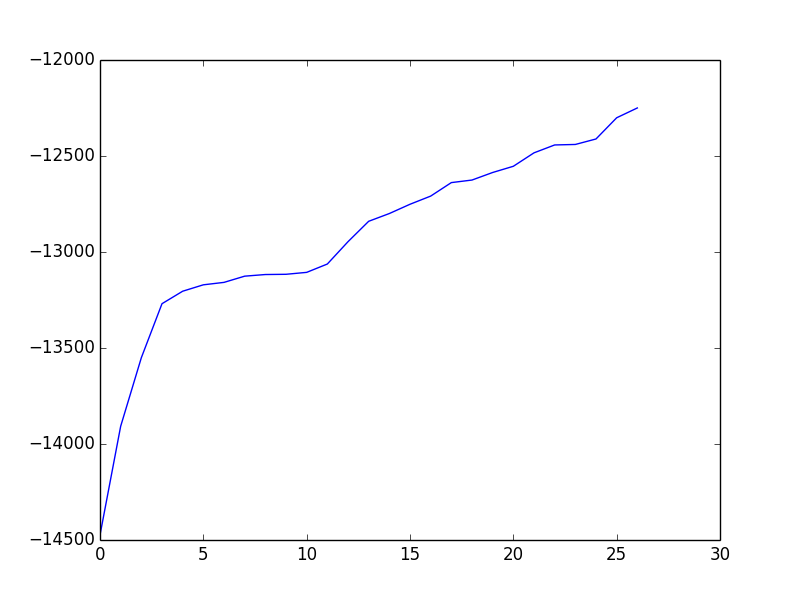
\includegraphics[width=0.4\columnwidth]{figure_train.png}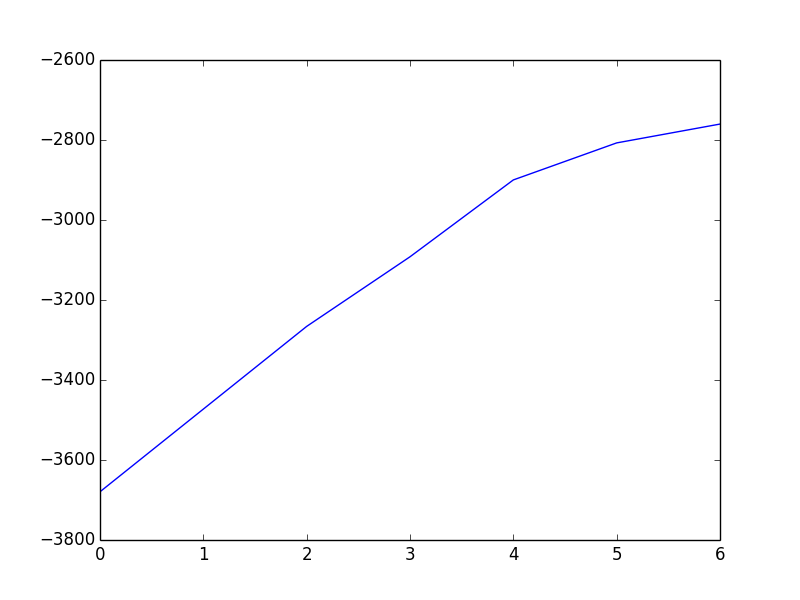
\includegraphics[width=0.4\columnwidth]{figure_test.png}

Note that I didn't include the initial likelihood in the grammar since the first iteration has a big jump, which makes the rest changes indistinguishable in the figure.

\item In my solution for this first type of randomization, I pick $\mu_k$ for each feature $k$ is sample from a uniform distribution between ranges $[\mathit{min}_k, \mathit{max}_k]$, where $\mathit{min}_k$ and $\mathit{max}_k$ are min-max values for the $k$-th feature of all data in the dataset. With this way of sampling, two methods works roughly the same. The reason is that both methods similar chances to hit the real means for each class.

\item When I ran 10 times, the log likelihood stays pretty similar. The values are
$-12255.503663$, $-12255.503663$, $-12442.4946406$, $-12255.503663$, $-12688.6646817$, $-12688.6646745$, $-12159.5228952$, $-12186.985494$, $-12688.6646745$, $-12254.5239628$, $-12121.9834305$.

\item Our algorithm is able to classify 103 out of 142 correct. Major faults are result from the difficulties in distinguishing the first and the third types of wines.

\item The figure for different clustering is shown below. 

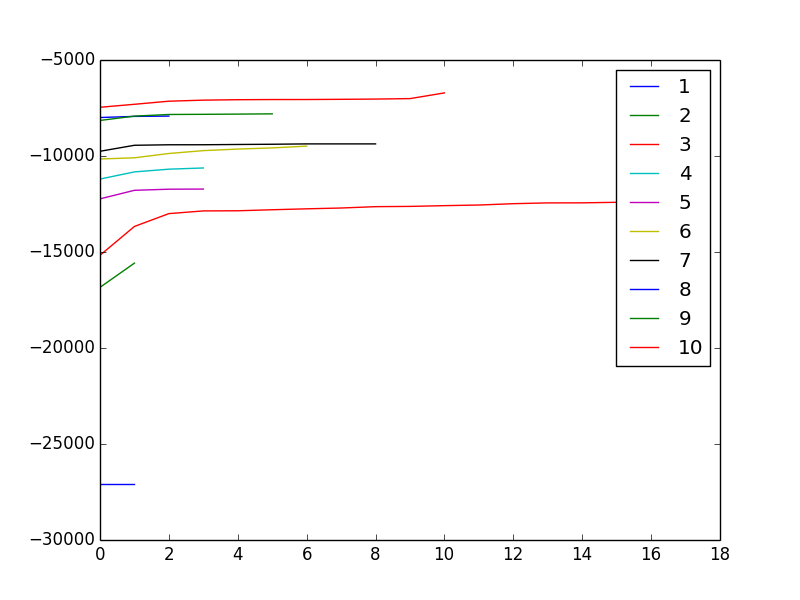
\includegraphics[width=0.7\columnwidth]{different_cluster.png}

I noticed that 3 clusters contains best likelihood, while given 1 is the worst. The reason for that is that having more or less clusters tend to make the model overfit to training data, and the result is less satisfying likelihood.

\end{enumerate}


\end{document}